\subsection{Dns Script}
\begin{figure}[htp]
\centering
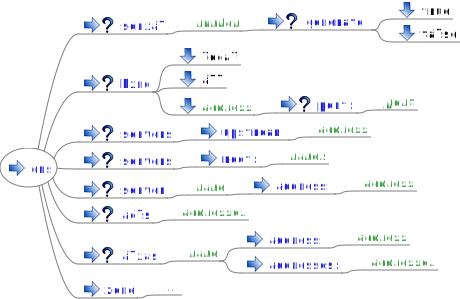
\includegraphics[angle=90,height=0.7\textheight]{dns_service_script}
\label{fig:dns_script_statements}
\caption{Dns Script Statements}
\end{figure}


\TheStatement{dns}
\TheStatement*[dns]{dns \{ serial bind alias roots recursive zone \}}

Entry point in the dns script.

\TheStatement[dns:serial]{serial}
\TheStatement*[dns!serial]{serial \Arg{number} [, generate: true|false]}

Sets the serial \Arg{number} of the zone records.
The serial number can be any number, it is added to the automatically
generated serial. The DNS service needs the serial number to be updated
for all records that have been changed. The service can create serial
numbers based on the current date but the user needs to update this
serial number if the records are changed more then once in a day.
If generate is set to \code{true} then the serial number is added to
the automatically generated serial, otherwise the serial number is used 
as specified.

\TheStatement[dns:bind]{bind}
\TheStatement*[dns!bind]{bind [address: [local|all|\Arg{address}] [, addresses: \Arg{addresses}]}

The IP \Arg{address} or a list of \Arg{addresses} or the host name(s) 
on which the dns server should listen to connections. Set to \qcode{local}
for the local host address \code{127.0.0.1} or to \qcode{all} to listen to all
hosts.

% alias
\TheStatement[dns:alias]{alias}
\TheStatement*[dns!alias]{alias \Arg{name} address \Arg{address}}

Sets alias \Arg{name} for the specified \Arg{address}. Can be used multiple times
for different aliases.

% roots
\TheStatement[dns:roots]{roots}
\TheStatement*[dns!roots]{roots { servers }}

Sets the servers as the root servers.

% servers
\TheStatement[dns:roots:servers]{servers}
\TheStatement*[dns!roots!servers]{servers { servers \Arg{name} }}

Sets servers group \Arg{name} as the root DNS servers. The group name is
an alias for IP addresses that are defined.

% recursive
\TheStatement[dns:recursive]{recursive}
\TheStatement*[dns!recursive]{recursive { servers }}

Allow the servers recursive look-up.

% servers
\TheStatement[dns:recursive:servers]{servers}
\TheStatement*[dns!recursive!servers]{servers { servers \Arg{name} }}

Allow for servers \Arg{name} recursive look-up. The servers name is an alias
for the IP addresses or host names that were defined previosly.

\TheStatement[dns:zone]{zone}
\TheStatement*[dns!zone]{zone \Arg{name}, primary: \Arg{primary}, email: \Arg{email} [, serial: \Arg{serial}]}\\
\TheStatement*{[, address: \Arg{address}] [, ttl: \Arg{time}] [, \{ ttl refresh retry}\\
\TheStatement*{expire record \} ]}

Adds a new DNS zone. The \Arg{name}, the \Arg{primary} DNS server and 
the \Arg{email} address of the zone are required. The \Arg{serial} number can
be set for the DNS zone.
An A-record for the zone
can be created if the IP \Arg{address} of the zone is specified. If the
TTL \Arg{time} is specified it is set for the A-record.

\TheStatement[dns:ttl]{ttl}
\TheStatement*[dns!ttl]{ttl duration: \Arg{duration} [, minimum: \Arg{duration}]}

Sets the time to live \Arg{duration}. 
The duration accept ISO 8601 time formats.

\TheStatement[dns:refresh]{refresh}
\TheStatement*[dns!refresh]{refresh duration: \Arg{duration}}

Sets the refresh time \Arg{duration}.
The duration accept ISO 8601 time formats.

\TheStatement[dns:retry]{retry}
\TheStatement*[dns!retry]{retry duration: \Arg{duration}}

Sets the retry time \Arg{duration}.
The duration accept ISO 8601 time formats.

\TheStatement[dns:expire]{expire}
\TheStatement*[dns!expire]{expire duration: \Arg{duration}}

Sets the expire time \Arg{duration}.
The duration accept ISO 8601 time formats.

\TheStatement[dns:record]{record}
\TheStatement*[dns!record]{record a|ns|mx|cname [, name: \Arg{name}] [, alias: \Arg{alias}]}\\
\TheStatement*{[, address: \Arg{address}] [, priority: \Arg{priority}] [, \{ ttl \}]}

Adds a new DNS record to the DNS zone. 
The accepted arguments are depending on
the record type. The \qcode{a} record type will add a new A-record with the 
specified \Arg{name} and \Arg{address}; 
the \qcode{ns} record type will add a 
new NS-record with the specified \Arg{name}. If 
the \Arg{address} of the NS-record is specified then a new A-record will be 
created that maps this name to the specified address and uses the 
same TTL duration;
the \qcode{mx} record type will add a 
new MX-record with the specified \Arg{name}. Optionally, the \Arg{priority}
of the MX-record can be set. If the \Arg{address} of the MX-record is 
specified then a new A-record will be created that maps this name to the 
specified address and uses the same TTL duration;
the \qcode{cname} record type will add
a new CNAME-record with the specified \Arg{name} and \Arg{alias}.
The placeholder \qcode{\%} can be used that is replaced by the current zone.
